This chapter presents the design and implementation of \bpfbox{}, an initial research
prototype of an \gls{ebpf}-based confinement framework. \bpfbox{} is the first
full-fledged confinement framework to leverage \gls{krsi}'s \gls{lsm} programs to enforce
high-level policy. Using \gls{ebpf}, it combines various behavioural aspects of the
sandboxed application from both userspace and kernelspace to enforce a simple, yet
fine-grained policy defined in a domain-specific policy language. This chapter was a part
of a previously published paper at CCSW'2020, co-authored with Anil Somayaji and David
Barrera~\cite{findlay2020_bpfbox}.



\section{\bpfbox{} Overview}

At a high level, \bpfbox{} is a confinement mechanism based on \gls{ebpf}. As outlined in
\Cref{s:cp-design} of \Cref{c:confinement-problem}, our primary design goals are
simplicity, flexibility, suitability for containerized applications, and flexibility. With
this in mind, \bpfbox{} attempts to be as light-weight as possible, with a simple policy
language that supports optional granularity. Perhaps the most important goal of \bpfbox{}
may be derived from the aforementioned goals: to make per-application security policy
accessible to end-users. To achieve these goals, we leverage \gls{ebpf} for \bpfbox{}'s
kernelspace implementation and rely on a number of its intrinsic properties.

In particular, we take advantage of multiple program and map types (outlined in
\Cref{ss:bpfbox-architecture}). This design enables us to trace multiple aspects of system
behaviour, including userspace and kernel function calls, and combine these with
\gls{lsm}-layer enforcement, thanks to the \gls{krsi} extension that enables \gls{bpf}
programs to be attached to \gls{lsm} hooks. By sharing data across program types in this
way, we enable \bpfbox{} to define extremely fine-grained \gls{lsm} policy at the
per-function-call level, something which no existing process confinement mechanism can do.

Since \gls{ebpf} programs may be loaded dynamically into a vanilla kernel and provide
implicit safety guarantees thanks to the verifier, we ensure that \bpfbox{} is both
light-weight and more adoptable than conventional solutions based in static \glspl{lsm}
like SELinux or AppArmor. Since all of \bpfbox{}'s kernelspace code is pre-verified, it is
also significantly less likely to adversely affect a production kernel than an alternative
solution implemented as a kernel patch or kernel module.

Whereas the kernelspace components are implemented using \gls{ebpf} programs written in C,
\bpfbox{}'s userspace components are implemented in Python3. In particular, this consists
of a privileged daemon loads \bpfbox{}'s \gls{ebpf} programs and maps into the kernel,
manages their lifecycle, and logs policy enforcement actions for later examination.

% This daemon is implemented in bcc~\cite{bcc}, a Python3 library that acts as
% a userspace \gls{ebpf} front-end.  bcc in turn is based on libbpf~\cite{libbpf} and uses
% the LLVM toolchain~\cite{llvm_bpf} to compile its \gls{bpf} programs at runtime before
% they can be loaded into the kernel.

\subsection{Policy Enforcement at a High Level}%
\label{ss:bpfbox-enforcement-overview}

To confine an application, a user first authors a high-level policy written in \bpfbox{}'s
domain-specific policy language (outlined in \Cref{s:bpfbox-policies}). The policy
language is designed in such a way as to permit the authorship of simple confinement
policies while offering the ability to augment them with specific context. Thus, the user
has full control over the balance between policy expressiveness and policy simplicity. We
expect that application authors may wish to take advantage of \bpfbox{}'s full
expressiveness, whereas end-users may wish to overlook advanced features in favour of
simple, light-weight confinement policy.

Once a policy has been written, the user places it in a pre-determined policy directory
and loads \texttt{bpfboxd}, the \bpfbox{} daemon. The daemon compiles and loads its
\gls{bpf} programs and maps into the kernel, then parses the user-supplied policy and
encodes it into policy maps. When a user launches the target application, \bpfbox{} begins
tracing the lifecycle of the corresponding processes and associates them with the correct
policy. As the application runs, \bpfbox{} continually updates security-critical aspects
of its state, stored in intermediary maps. As the application makes requests to sensitive
resources, \bpfbox{} queries policy maps and state maps and uses this information to come
to an enforcement decision. \Cref{fig:bpfbox-policy-overview} outlines this process in full.

\begin{figure}[htpb]
  \centering
  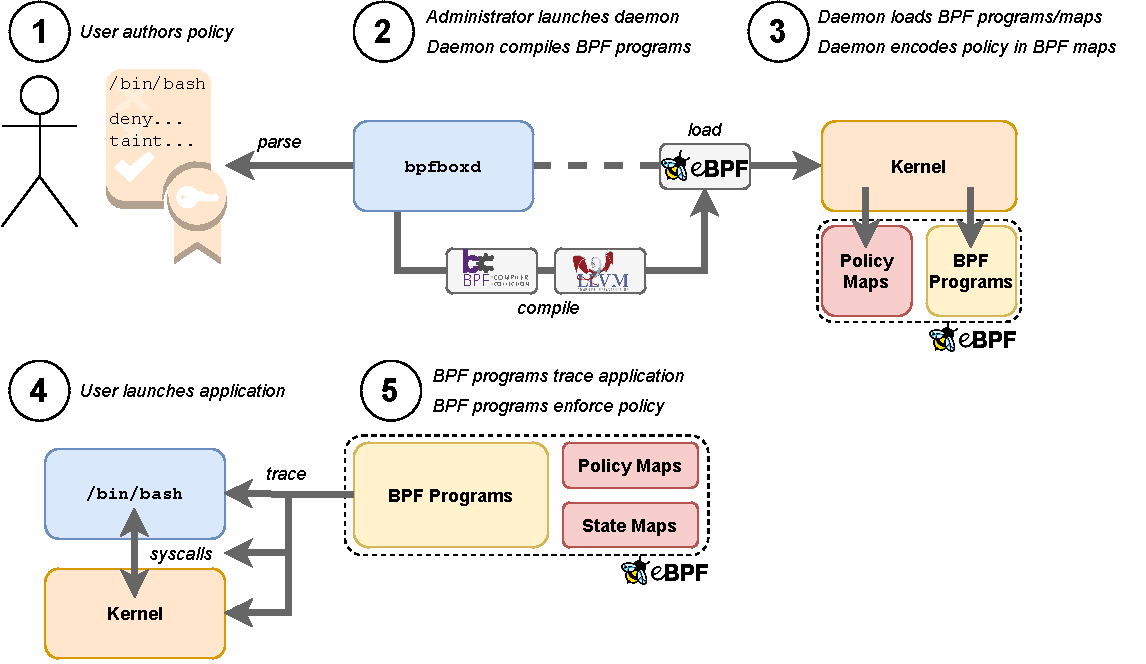
\includegraphics[width=0.8\linewidth]{figs/bpfbox/overview.pdf}
  \caption[A high-level overview of how \bpfbox{} confines applications]{
    A high-level overview of how \bpfbox{} confines applications. Users write policy files
    which the daemon encodes into \gls{ebpf} maps. The daemon loads these maps, along with
    policy enforcement and tracing programs into the kernel. At runtime, \bpfbox{}'s
    \gls{bpf} programs trace the application and enforce policy.
  }%
  \label{fig:bpfbox-policy-overview}
\end{figure}



\section{\bpfbox{} Implementation}%
\label{s:bpfbox-implementation}

This section presents the implementation details and full architecture of \bpfbox{}.  In
particular, we provide an architectural overview and discuss \bpfbox{}'s policy
enforcement implementation, along with how it tracks and manages the state and lifecycle
of sandboxed processes. We focus specifically on implementation details here, leaving
policy language design and documentation to \Cref{s:bpfbox-policies}.

\subsection{Architectural Overview}%
\label{ss:bpfbox-architecture}

In userspace, \bpfbox{} runs as a privileged daemon (\texttt{bpfboxd}), implemented in
Python3 using the bcc~\cite{bcc} userspace library for \gls{ebpf}. The daemon uses the
LLVM toolchain~\cite{llvm_bpf} to compile \gls{ebpf} programs which are then loaded into
the kernel using bcc-provided wrappers around the \texttt{bpf(2)} system call. The daemon
provides a userspace front-end to \bpfbox{}, managing the lifecycle of its \gls{bpf}
programs and maps and logging security-sensitive events as they occur. To load policy into
the kernel, \texttt{bpfboxd} implements a full parser and lexer for \bpfbox{}'s custom
policy language.  After parsing policy, \texttt{bpfboxd} encodes it into a format that can
be subsequently loaded into kernelspace through \gls{bpf} maps.

\bpfbox{}'s kernelspace components are implemented in \gls{ebpf} and based on several
\gls{bpf} program and map types, summarized as follows. Maps are outlined in
\textbf{\green{green}} and programs are outlined in \textbf{\purple{purple}}. The reader
is encouraged to revisit \Cref{ss:bpf-programs-bg,ss:bpf-maps-bg} in \Cref{c:background},
where necessary, for clarification on specific program and map types.

\begin{itemize}
  \item \bpfbox{} uses \textbf{\green{Hashmaps}} to store runtime state, share state
  between its \gls{bpf} programs, and communicate with the userspace daemon. In
  particular, \bpfbox{} maintains a set of hashmaps to store per-process state and a set
  of hashmaps to store policy. We call these \textit{state maps} and \textit{policy maps}
  respectively.  At runtime, \bpfbox{}'s \gls{lsm} programs query these state maps and
  policy maps to make enforcement decisions.

  \item \textbf{\green{Ringbufs}} provide \bpfbox{}'s \gls{bpf} programs with a canonical
  data store to push per-event audit data to userspace. In the kernel, the ringbuf map is
  implemented as a circular buffer that is efficiently shared across all \glspl{cpu}.
  In userspace, the \bpfbox{} daemon maps the ring buffer into memory and continually
  polls for new events over a fixed interval.
  % \item \textbf{State Maps} are \gls{ebpf} hash maps that associate a kernel \gls{tid}
  % with a specific task state. The task state holds information including policy
  % association, task liveness, and other metadata used for enforcement.

  % \item \textbf{Policy Maps} are \gls{ebpf} hash maps that encode \bpfbox{} policy for
  % various categories of access. Each map encodes an access vector and policy ID pair that
  % is mapped to the corresponding enforcement decision. At runtime, \bpfbox{} queries these
  % maps before making an enforcement decision on a specific access pattern.

  \item \textbf{\purple{Tracepoints}} enable \bpfbox{} to track the state of a process from the
  point where it forks or executes a new binary to when it exits. \bpfbox{} stores
  per-process state from its tracepoints in \textit{state maps} for later use.

  \item \textbf{\purple{\gls{lsm} Probes}} enforce policy by attaching to \gls{lsm} hooks in the
  kernel. These hooks are called by kernel functions such as system call implementations
  and trigger the corresponding \gls{bpf} program, which enforces a policy decision on the
  target application. To enforce policy, \bpfbox{}'s \gls{lsm} probes query \textit{policy
  maps} and \textit{state maps}.

  \item \textbf{\purple{Kprobes and Uprobes}} are used to enforce \textit{stateful policy},
  according to what function calls a process has made, in kernelspace and userspace
  respectively. A \bpfbox{} policy file may outline that certain rules should only apply
  within the context of a specific function call; when a process runs some code that
  results in such a function call, the corresponding kprobe or uprobe will make an update
  to the process' \textit{state map} to indicate this. \bpfbox{} then considers this state
  when making later enforcement decisions.

  \item \textbf{\purple{\gls{usdt} Probes}} form the backbone of \textit{libbpfbox},
  providing a kernel-side implementation for various \enquote{commands}. Commands are
  implemented in userspace as stub \gls{usdt} functions that trap to a kernelspace
  \gls{usdt} program. These are used to load policy into the kernel and perform various
  other interactions between the daemon and its \gls{bpf} programs and maps.
\end{itemize}

\subsection{\bpfbox{} Policy Enforcement}%
\label{ss:bpfbox-enforcement}

\bpfbox{} policies are written using a custom policy language.  \bpfbox{}'s policy
language supports three distinct policy decisions for a given rule; the operation may be
allowed, audited (logged), and/or tainted.  Any unspecified operations are denied by
default. Tainting is similar in spirit to Perl's classic taint mode~\cite{hurst2004_perl},
however, rather than marking data, it marks the entire process.  Tainting allows for more
restrictive policies to be enforced once a process has engaged in specific unsafe
operations, say by reading from a network socket.  We present the design and syntax of the
\bpfbox{} policy language in \Cref{s:bpfbox-policies}; here we discuss the functionality
it provides and how it is implemented.

\bpfbox{} policies are per-executable and are stored in an exclusively root-controlled
directory (by default, \texttt{/var/lib/bpfbox/}), written in \bpfbox{}'s policy language
(c.f.~\Cref{s:bpfbox-policies}). When an executable is loaded, \bpfbox{} loads the corresponding
policy file (if it exists) and translates it into a series of function calls to \gls{usdt}
stub functions.  These function calls trigger the corresponding \gls{ebpf} code, thus recording
the policy in the policy maps as a set of policy structures.  A policy structure consists
of three distinct access vectors: one to define tainting operations, one to define allowed
operations, and one to define audited operations.

In order to enforce policy, \bpfbox{} leverages the KRSI patch by KP
Singh~\cite{singh2019_krsi, corbet2019_krsi} which was upstreamed in Linux
5.7. This patch provides the necessary tools to implement MAC policies in \gls{ebpf} by
instrumenting probes on \gls{lsm} hooks provided by the kernel. The \gls{ebpf} program can then
audit the event and optionally enforce policy by returning a negative error value.
\bpfbox{} instruments several \gls{lsm} probes covering filesystem access, \gls{ipc}, network
sockets, \texttt{ptrace(2)}, and even \texttt{bpf(2)} itself.  When these hooks are
called in the kernel, they trigger the execution of the associated \gls{ebpf} program which
is, in general, composed of the following six steps:
\begin{enumerate}
\item Look up the current process state.  If no state is found, the process is
      not being traced, so \textbf{grant access}.
\item Determine the \textit{policy key} by taking the executable's inode
      number and filesystem device number together as a struct.
\item Look up the policy corresponding to the \textit{policy key} calculated in step (2). If the
      process is \textit{tainted} and no such policy exists, \textbf{deny access}.
\item If the process is \textit{not tainted} and the current access corresponds to
      a \textbf{taint rule}, \textbf{taint} the process and \textbf{grant access}.
\item If the current access matches an \textbf{allow rule}, \textbf{grant access}.
      Otherwise \textbf{deny access}.
\item If the current access matches an \textbf{audit rule} or access is \textbf{denied},
      submit an \textit{audit event} to userspace.
\end{enumerate}

%\Cref{fig:bpfbox-enforcement} depicts \bpfbox{}'s mediation of a request
%to a security-sensitive resource.

When a sandboxed application requests access, a corresponding \gls{lsm} hook is called which in
turn traps to one or more of \bpfbox{}'s \gls{lsm} probes. The probe queries the state of the
currently running process along with the policy corresponding to the requested access and
takes these factors together to come to a policy decision.

%% \begin{figure}[tpb]
%%     \centering
%%     \includegraphics[width=1\linewidth]{figs/bpfbox-enforcement.png}
%%     \caption{\bpfbox{}'s mediation of a security-sensitive operation.
%%     Security-sensitive operations by sandboxed applications trap to an
%%     \gls{lsm} hook which in turn invokes the corresponding BPF \gls{lsm} probe to
%%     query and enforce policy.
%%     }%
%%     \label{fig:bpfbox-enforcement}
%% \end{figure}

\bpfbox{} can optionally augment the information provided by the \gls{lsm} hooks themselves with
additional context obtained by instrumenting other aspects of process behaviour. For
instance, profiles may optionally define \textit{function contexts} which determine the
validity of specified rules; a rule could specify that a certain filesystem access must
occur within a call to the function \texttt{foo()} or that it must be audited within
a call to the function \texttt{bar()}. The ability to combine various aspects of system
behaviour, both in kernelspace and in userspace, is a key advantage of an \gls{ebpf}-based
solution over traditional techniques. This allows for the creation of extremely
fine-grained policies at the discretion of the policy author. The mechanisms by which this
is accomplished are discussed further in \Cref{ss:bpfbox-state}.

Due to \bpfbox{}'s strict resolution of filesystem objects at policy load time, a problem
arises when dealing with applications that read or write temporary files on disk or create
new files at runtime. In order to circumvent this issue, \bpfbox{} treats the creation of
new files as a special case. In order for a new file to be created, the process must have
write access to the directory in which the files will be created.  Supposing, for
instance, the temporary file would be written to \texttt{/tmp}, this means that, at
a minimum, the policy in question must specify that \texttt{/tmp} is writable.  When the
sandboxed application creates a new child inode of \texttt{/tmp}, \bpfbox{} dynamically
creates a temporary rule that grants the application full read, write, link, and unlink
capabilities on the created file. This rule is keyed using a combination of the standard
filesystem policy key and the PID (process ID) of the sandboxed process. This rule is then
automatically cleaned up when the process exits or transitions to a new profile.

Another important detail to consider is the possibility of other applications using the
\texttt{bpf(2)} system call to interfere with \bpfbox{}'s mediation of sandboxed
applications. For instance, another application might attempt to unload an \gls{lsm} probe
program or make changes to the policy or process state maps. To prevent this, \bpfbox{}
instruments an additional \gls{lsm} probe to mediate access to \texttt{bpf}. It uses this probe
to deny all calls to \texttt{bpf} that attempt to modify \bpfbox{}'s programs or maps that
do not directly come from \bpfbox{} itself. Further, all sandboxed applications are
strictly prohibited from making \textit{any} calls to \texttt{bpf}---a sandboxed
application has \textit{no business} performing the kind of powerful system introspection
that \gls{ebpf} provides.

Similarly to mandatory access control systems like SELinux~\cite{smalley2001_selinux} and
AppArmor~\cite{cowan2000_apparmor}, \bpfbox{} supports the ability to run in either a
\textit{permissive mode} or \textit{enforcing mode}.  When running in permissive mode,
\bpfbox{} continues to audit denied operations, but allows them to continue unobstructed.
This enables the user to debug policies before putting them into effect and also
introduces the possibility of creating new policy based on the generated audit logs.



\subsection{Managing Process State}%
\label{ss:bpfbox-state}

In order for \bpfbox{} to know what policy to apply to a given process, it must track the
lifecycle of processes through the instrumentation of key events within the kernel. For
this, \bpfbox{} uses three tracepoints exposed by the scheduler:
\texttt{sched:process\_fork}, \texttt{sched:process\_exec}, and
\texttt{sched:process\_exit}. \Cref{fig:bpfbox-process-lifecycle} shows the events that \bpfbox{}
instruments in order to track process state, along with their corresponding probe types.
These tracepoints are used to create, update, and delete per-task entries in a global
hashmap of \textit{process states}.  Each entry in the map is keyed by \gls{tid}. The
entries themselves consist of a data structure that tracks policy key association and
a 64-bit vector representing the \textit{state} of the running process.  This state vector
is used to track whether the process is currently tainted and what important function
calls are currently in progress.

\begin{figure}[htbp]
  \centering
  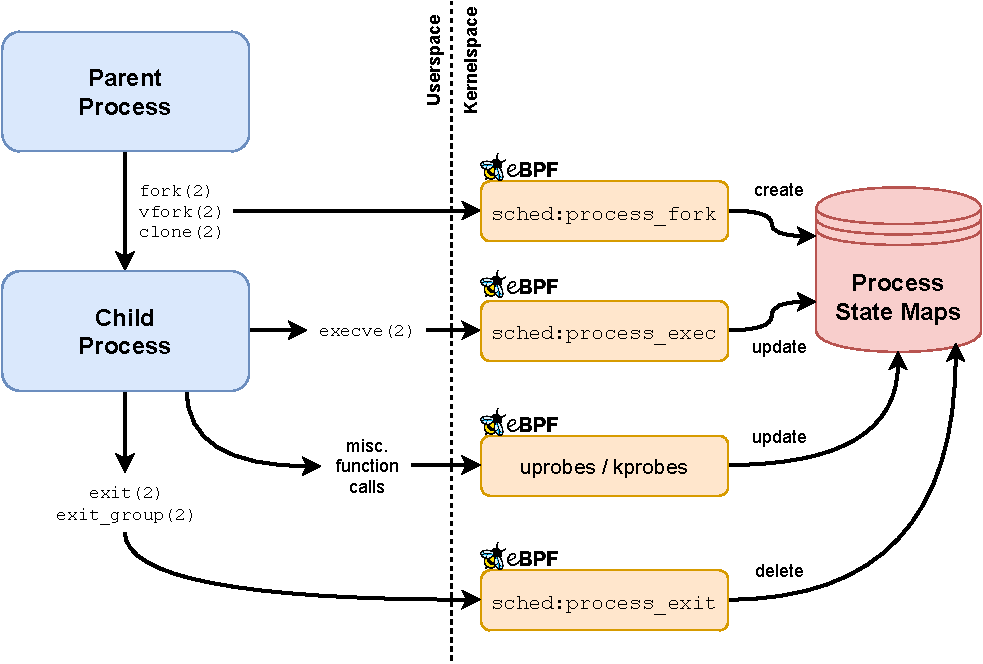
\includegraphics[width=0.8\linewidth]{figs/bpfbox/process-lifecycle.pdf}
  \caption[The various mechanisms that \bpfbox{} uses to manage process state]{
    The various mechanisms that \bpfbox{} uses to manage process state.
    Probes marked \texttt{sched:*} are tracepoints instrumenting scheduler events
    in the kernel. Uprobes and kprobes instrument userspace
    and kernelspace function calls respectively.
  }%
  \label{fig:bpfbox-process-lifecycle}
\end{figure}

%% \begin{lstlisting}[language=c, caption={The data structure stored in the \textit{process states} hashmap,
%% which \bpfbox{} uses to track the state of running tasks. The map is keyed by
%% thread ID.}, label={lst:process-state}]
%% struct bpfbox_process_t {
%%     /* Key of the profile associated with
%%      * this process. */
%%     u64 profile_key;
%%     /* A 64-bit vector representing
%%      * the current state of the process. */
%%     u64 state;
%% };
%% \end{lstlisting}

Instrumenting a tracepoint on \texttt{sched:process\_fork} allows \bpfbox{} to
detect when a new task is created via the \texttt{fork(2)}, \texttt{vfork(2)}, or
\texttt{clone(2)} system calls. This tracepoint creates an entry in the \textit{process
states} hashmap and initializes it according to the state of the parent process; if the
parent process is associated with a \bpfbox{} profile, its key is copied to the child
until such time as the child makes an \texttt{execve(2)} call.

The \texttt{sched:process\_exec} tracepoint is triggered whenever a task calls
\texttt{execve} to load a new program.  \bpfbox{} uses this tracepoint to manage the
association of \textit{policy keys} to a particular \textit{process state}.  \bpfbox{}
policy may optionally specify whether a transition from one profile to another may occur
in a given call to \texttt{execve}; this transition is disallowed by default.

Finally, the \texttt{sched:process\_exit} tracepoint allows \bpfbox{} to detect when
a task exits. This tracepoint deletes the corresponding entry in the \textit{process
states} map.

\subsection{Context-Aware Policy}
\label{ss:bpfbox-context-aware}

If the policy for a given executable defines specific function call contexts for
particular rules, \bpfbox{} instruments these function calls using uprobes (for userspace
functions) and kprobes (for kernelspace functions). Each instrumented function call is
associated with a unique bit in the process' \textit{state} bitmask.  A probe is triggered
on entry that causes \bpfbox{} to flip the corresponding bit to a \texttt{1}, and again on
return, flipping the corresponding bit back to a \texttt{0}.
\Cref{fig:bpfbox-function-calls} depicts how \bpfbox{} instruments userspace and
kernelspace function calls for policy enforcement.

\begin{figure}[p]
  \centering
  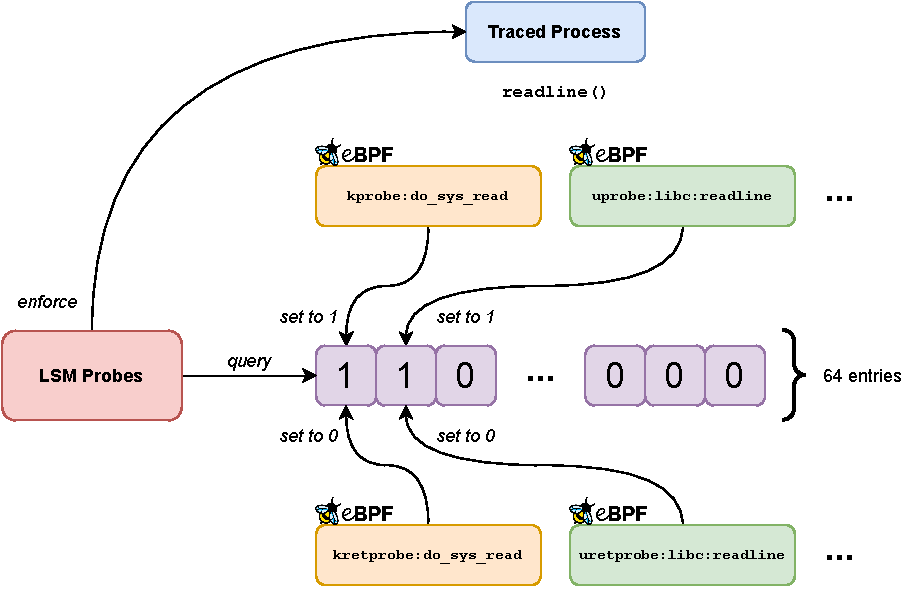
\includegraphics[width=1\linewidth]{figs/bpfbox/function-calls.pdf}
  \caption[How \bpfbox{} tracks function calls]{
    How \bpfbox{} uses kprobes and uprobes to track function calls.  If a policy
    identifies that a rule should apply within the context of a certain function call,
    \bpfbox{} instruments a probe on function entry and return. These probes flip the
    corresponding bit in the process' state vector, indicating to policy enforcement
    probes whether or not the process is in the middle of making the function call.
  }%
  \label{fig:bpfbox-function-calls}
\end{figure}

This approach is subject to a few inherent limitations.  Firstly, compile-time
optimizations such as function in-lining can invalidate the probe by removing the
corresponding symbol in the target object file. Secondly, a recursive call that is not
tail-optimized will break enforcement by prematurely signalling to \bpfbox{} that
a process has exited a given function context.  The first limitation may be trivially
worked around by hinting to the compiler that a given function should not be in-lined;
although this sacrifices some application transparency and incurs a slight performance
penalty, the potential security benefits from such a fine-grained policy are arguably
worth the trade-off.  The second limitation \textit{could} be worked around by maintaining
a reference counter for each function call rather than a flat vector. \bpfbox{} currently
does not do this, since it would incur a larger memory overhead for each active process,
but it would be possible to extend a future version of \bpfbox{} with this workaround. In
case working around these limitations is impractical, the policy author would simply fall
back to specifying ordinary rules rather than context-specific ones.



\subsection{Collecting and Logging Audit Data}%
\label{ss:bpfbox-audit}

When an operation is denied or matches with an audit rule, \bpfbox{} submits an event to
userspace for logging. To accomplish this, we leverage the new ringbuf map type added in
Linux 5.8. The \gls{ebpf} ringbuf map implements an efficient ring buffer that is shared
across all \glspl{cpu}. This new map type comes with a number of optimizations for fast
reads and writes and in-order guarantees for asynchronous events across multiple
\glspl{cpu}, allowing per-event data to be efficiently shared with userspace in near
real-time.

In userspace, the \bpfbox{} daemon uses \texttt{mmap(2)} to map the corresponding memory
region and polls for new data at regular intervals. As events are consumed in userspace
they are removed from the ring buffer to make room for new events.  Since the ringbuf map
provides strong order guarantees and high performance under contention, we can ensure that
\bpfbox{} always provides highly reliable and performant per-event auditing.



\section{\bpfbox{} Policy Language}%
\label{s:bpfbox-policies}

\bpfbox{} policies are a series of rules and accompanying decorators. A decorator may
annotate either individual rules or blocks of rules denoted by braces and is used to
specify additional context or policy actions. The first line in a \bpfbox{} policy is
always a special \enquote{profile decorator}, written as
\lstinline[language=bpfbox]{#![profile "/path/to/exe"]}, which marks the executable to
which the policy should be associated.  Other than the profile decorator, all others take
the form of \lstinline[language=bpfbox]|#[decorator] { rule() }|. Multiple decorators may
be specified before a set of rules, meaning that all decorators apply to each rule.

Profile assignment occurs when a process makes an \texttt{execve(2)} call that results in
loading the specified executable.  Once a process has been assigned a profile, this
profile cannot change again, unless an \texttt{execve(2)} occurs which has been explicitly
marked with the \lstinline[language=bpfbox]{#[transition]} decorator. This ensures that
policy transitions only occur when expected and prevents malicious \texttt{execve(2)}
calls from changing \bpfbox{}'s treatment of a process.

The sections that follow describe the rule categories supported by \bpfbox{}
(\Crefrange{ss:bpfbox-filesystem-rules}{ss:bpfbox-ptrace-rules}) and the decorators that
may optionally be used to augment them (\Crefrange{ss:bpfbox-allow}{ss:bpfbox-kfunc}).
\Cref{lst:bpfbox-policy-example} depicts a simple example \bpfbox{} policy.

\begin{lstlisting}[language=bpfbox, gobble=4,
  caption={[An example \bpfbox{} policy]
    An example \bpfbox{} policy for a simple remote login program. This example offers
    a fairly complete idea of the \bpfbox{} policy language's various features.
  },
  label={lst:bpfbox-policy-example}, float]
    /* This policy applies to the /usr/bin/mylogin
     * executable */
    #![profile "/usr/bin/mylogin"]

    /* Taint process state upon binding to
     * any IPv4/IPv6 network socket */
    #[taint] {
      net(inet,  bind)
      net(inet6, bind)
    }

    /* Allow network connections/operations */
    #[allow] {
      net(inet,  accept|listen|send|recv)
      net(inet6, accept|listen|send|recv)
    }

    /* Allow the check_login function to read
     * /etc/passwd and /etc/shadow */
    #[func "check_login"] {
      fs("/etc/passwd", read)
      fs("/etc/shadow", read)
    }

    /* Allow the add_user function to read
     * and append to /etc/passwd, but log such
     * events to the audit logs */
    #[func "add_user"]
    #[audit] {
      fs("/etc/passwd", read|append)
    }

    /* Read and append to any immediate child
     * of the /var/log/mylogin/ directory */
    fs("/var/log/mylogin/*", read|append)

    /* Allow the execution of /bin/bash, transitioning
     * profiles to bash's profile after the execve(2)
     * and untainting the process */
    #[transition]
    #[untaint] {
      fs("/bin/bash", read|exec)
    }
\end{lstlisting}



\subsection{Filesystem Rules}%
\label{ss:bpfbox-filesystem-rules}

Filesystem rules in \bpfbox{} govern what operations a process may perform on filesystem
objects such as files and directories. They are written as
\lstinline[language=bpfbox]{fs("pathname", access)} where
\lstinline[language=bpfbox]{"pathname"} is a string containing the pathname of the file
and \lstinline[language=bpfbox]{access} is a list of one or more file access permissions
joined by the vertical bar symbol.  For instance, to represent read and
append permissions on \texttt{/var/log/my\_log}, the corresponding \bpfbox{} rule would be
\lstinline[language=bpfbox]{fs("/var/log/my_log", read|append)}.  In total, \bpfbox{}
supports nine distinct filesystem access flags as shown in \Cref{tab:fs-access}.

\begin{table}[htpb]
    \centering
    \caption{The filesystem access flags supported in \bpfbox{}.}
    \label{tab:fs-access}
    \begin{tabular}{lp{0.7\linewidth}}
    \toprule
    Flag & Meaning \\
    \midrule
    \texttt{read}    & The subject may read the object. \\
    \texttt{write}   & The subject may write to the object. \\
    \texttt{append}  & The subject may append to the object. \\
    \texttt{exec}    & The subject may execute the object. \\
    \texttt{setattr} & The subject may change the object's filesystem attributes. \\
    \texttt{getattr} & The subject may read the object's filesystem attributes. \\
    \texttt{rm}      & The subject may remove the object's inode. \\
    \texttt{link}    & The subject may create a link to the object's inode. \\
    \texttt{ioctl}   & The subject may perform an ioctl call on the object. \\
    \bottomrule
    \end{tabular}
\end{table}

\bpfbox{} supports a limited globbing syntax when defining pathnames, allowing multiple
rules matching similar files to be combined into one.  Although filesystem rules are
specified using pathnames, \bpfbox{} internally uses inode and device numbers rather than
the pathnames themselves. When loading policies, \bpfbox{} automatically resolves the
provided pathnames into their respective inode-device number pairs. This information is
then used to look up the correct policy whenever a sandboxed application attempts to
access an inode.  Since \bpfbox{} does not check the pathnames themselves when referring
to files, it is able to defeat \glsentryfull{toctou} attacks, where an
attacker quickly swaps out one file with a link to another in an attempt to circumvent
access control restrictions in a privileged (most often setuid)
binary~\cite{bishop1996_checking}.  In such a situation, \bpfbox{} would simply see
a different inode and deny access.

In addition to regular filesystem rules, \bpfbox{} provides a special rule type for
\texttt{/proc/pid} entries in the \texttt{procfs} virtual filesystem. \texttt{procfs}
rules, written as \lstinline[language=bpfbox]{proc("exe", access)} where
\lstinline[language=bpfbox]{"exe"} is a string containing the pathname of another
executable and \lstinline[language=bpfbox]{access} is the desired access. For example,
read-only access to the \texttt{procfs} entries of executables running
\texttt{/usr/bin/ls} may be specified with \lstinline[language=bpfbox]{proc("/usr/bin/ls", read)}.
Access to any \texttt{procfs} entry may be specified using the special keyword
\lstinline[language=bpfbox]{any}.



\subsection{Network Rules}%
\label{ss:bpfbox-network-rules}

\bpfbox{} implements networking policy at the socket level, covering both Internet sockets
as well as Unix domain sockets. Networking rules are specified using
\lstinline[language=bpfbox]{net(protocol, access)}, where
\lstinline[language=bpfbox]{protocol} is a networking protocol like \texttt{inet},
\texttt{inet6}, or \texttt{unix} and \lstinline[language=bpfbox]{access} is a list of
socket operations (\Cref{tab:net-access}) separated by vertical bars. For example, a rule
targeting \texttt{bind}, \texttt{accept}, and \texttt{connect} operations on an
\texttt{inet6} socket would look like \lstinline[language=bpfbox]{net(inet6, bind|connect|accept)},
while a rule targeting \texttt{create} operations on a \texttt{unix} socket would look
like \lstinline[language=bpfbox]{net(unix, create)}.

\begin{table}[htpb]
    \centering
    \caption{The socket operation flags supported in \bpfbox{}.}
    \label{tab:net-access}
    \begin{tabular}{lp{0.7\linewidth}}
    \toprule
    Flag & Meaning \\
    \midrule
    \texttt{connect}  & Subject may connect a socket to a remote address. \\
    \texttt{bind}     & Subject may bind a socket to a local address. \\
    \texttt{accept}   & Subject may accept an incoming socket connection. \\
    \texttt{listen}   & Subject may listen for incoming socket connections. \\
    \texttt{send}     & Subject may send messages over a socket. \\
    \texttt{recv}     & Subject may receive messages over a socket. \\
    \texttt{create}   & Subject may create new sockets. \\
    \texttt{shutdown} & Subject may shut down a socket connection. \\
    \bottomrule
    \end{tabular}
\end{table}



\subsection{Signal Rules}%
\label{ss:bpfbox-signal-rules}

Specifying signal behaviour in \bpfbox{} is done using the
\lstinline[language=bpfbox]{signal("exe", access)} where
\lstinline[language=bpfbox]{"exe"} is the pathname of another executable and
\lstinline[language=bpfbox]{access} is a list of signals allowed to be sent, separated by
vertical bars. Normally, only processes running the executable
\lstinline[language=bpfbox]{"exe"} are allowed to be signalled, but the special keyword
\lstinline[language=bpfbox]{any} may be used instead to specify the ability to signal
\textit{any} process on the system. Two additional keywords,
\lstinline[language=bpfbox]{parent} and \lstinline[language=bpfbox]{child}, allow parent
and child processes to be signalled instead.  The \lstinline[language=bpfbox]{access}
argument supports any Linux signal, in addition to a few helper keywords that can be used
to specify broad categories, such as \lstinline[language=bpfbox]{fatal} for fatal signals
and \lstinline[language=bpfbox]{nohandle} for signals that cannot be handled.  For
example, to specify the ability to send fatal signals to any process running
\texttt{/usr/bin/ls}, the corresponding \bpfbox{} rule would be
\lstinline[language=bpfbox]{signal("/usr/bin/ls", fatal)}.  To narrow permissions such
that only \texttt{SIGTERM} and \texttt{SIGINT} are allowed,
\lstinline[language=bpfbox]{signal("/usr/bin/ls", sigterm|sigint)} could be used instead.



\subsection{Ptrace Rules}%
\label{ss:bpfbox-ptrace-rules}

Just like with signals, \texttt{ptrace} access is specified as
\lstinline[language=bpfbox]{ptrace("exe", access)}, where
\lstinline[language=bpfbox]{access} is a list of allowed \texttt{ptrace} modes separated
by vertical bars. The \lstinline[language=bpfbox]{child} keyword is also available for
\texttt{ptrace} rules to allow tracing of any child process, regardless of the child's
current profile. For instance, a rule that allows a process to read and attach to a child
process would be written as \lstinline[language=bpfbox]{ptrace(child, read|attach)}, while
a rule that allows only read access to processes running \texttt{/usr/bin/ls} would be
written as \lstinline[language=bpfbox]{ptrace("/usr/bin/ls", read)}.  Note that currently
\texttt{ptrace} rules do not override other \texttt{ptrace} restrictions, such as those
imposed by Yama~\cite{yama}.



\subsection{Allow, Taint, and Audit Decorators}%
\label{ss:bpfbox-allow}

\bpfbox{} supports three distinct decorators for defining \textit{actions} that should be
taken when a given access matches a rule. The \lstinline[language=bpfbox]{#[allow]}
decorator causes \bpfbox{} to allow the access; however, it is not typically necessary to
explicitly specify this as undecorated rules are assumed to be allowed by default.
Regardless, it may be desirable to decorate such rules with
\lstinline[language=bpfbox]{#[allow]} to improve the clarity of the policy.
\lstinline[language=bpfbox]{#[taint]} is used to mark a rule as a \textit{taint rule},
which causes the process to enter a tainted state when matched. These rules can be thought
of as gateways into the rest of the policy.  Once a process is tainted, this cannot be
reversed unless it makes an \texttt{execve(2)} call explicitly marked with
\lstinline[language=bpfbox]{#[untaint]}.  Finally, \lstinline[language=bpfbox]{#[audit]}
may be combined with \lstinline[language=bpfbox]{#[allow]} to cause \bpfbox{} to log the
matching operation to its audit logs. This can be useful for marking rare behaviour that
should be investigated or for determining how often a given rule is matched in practice.



\subsection{Func and Kfunc Decorators}%
\label{ss:bpfbox-kfunc}

One of the key features of \bpfbox{} is the ability to specify specific application-level
and kernel-level context for rules. In the policy language, this is done by decorating
rules with the \lstinline[language=bpfbox]{#[func "fn_name" ("filename")]} and
\lstinline[language=bpfbox]{#[kfunc "fn_name"]} decorators for userspace and kernelspace
instrumentation respectively. Here, \lstinline[language=bpfbox]{"fn_name"} refers to the
name of the function to be instrumented and \lstinline[language=bpfbox]{"filename"} refers
to the filename where the function symbol should be looked up --- this parameter is
optional and allows for the instrumentation of shared libraries.  These decorators provide
powerful tools for defining extremely fine-grained, sub-application level policy. For
instance, to declare that read access to the file \texttt{/etc/shadow} should only occur
during a call to the function \texttt{check\_password()}, the corresponding \bpfbox{} rule
would look like:
\begin{lstlisting}[language=bpfbox]
#[func "check_password"]
fs("/etc/shadow", read)
\end{lstlisting}
A process that is sandboxed using this policy would be unable to access
\texttt{/etc/shadow} except within a call to the specified function.



\section{Limitations and the Transition Toward \bpfcontain{}}%
\label{s:bpfbox-bpfcontain}

While \bpfbox{} certainly offers a new perspective on confinement and improves the status
quo, the extent to which it achieves the design goals outlined in \Cref{s:cp-design} is
arguably hampered by a few inherent limitations. We address these limitations in its
successor, \bpfcontain{}, the design of which is outlined in the next chapter. Before we
examine \bpfcontain{} in full, we first address the fundamental limitations of \bpfbox{}
as a confinement mechanism and offers some insights into how \bpfcontain{} addresses them.
\begin{enumerate}
  \item \textbf{Dependency Overhead and Runtime Overhead.}
    Due to its userspace implementation using bcc, \bpfbox{} has a high dependency
    overhead. This overhead is the combined result of a number of requirements imposed on
    the host system by the bcc toolchain. On the userspace side, bcc depends on Python as
    well as the entire LLVM toolchain for program compilation. Both of these are rather
    hefty requirements on their own. Python requires an entire language runtime, and
    a full LLVM toolchain can introduce gigabytes of additional code.

    Furthermore, Python and bcc incur significant runtime overhead. Python is an
    interpreted language with a much heavier runtime than compiled systems languages like
    C or Rust.  This runtime incurs additional performance disadvantages due to safety
    features like the global object lock, which impede concurrency. Since bcc compiles
    \gls{ebpf} programs at runtime, we incur additional compilation overhead for each
    program, sometimes resulting in significant startup delays depending on the complexity
    of the application. This runtime compilation also necessitates the availability of
    kernel headers as a compilation dependency in the target environment, adding further
    storage overhead.

    \bpfcontain{} solves these dependency and runtime overhead issues by leveraging Rust
    and libbpf \gls{core}~\cite{nakryiko2020_core} rather than Python and bcc.  Unlike
    bcc, libbpf \gls{core} enables \gls{bpf} programs to be compiled once and run
    anywhere, thanks to \gls{btf} information provided by the kernel and load-time symbol
    relocation. Program bytecode can then be embedded directly into the compiled object
    file, meaning the single pre-compiled \bpfcontain{} binary can be deployed on any
    target kernel that meets a minimal set of requirements. As a side effect,
    \bpfcontain{} requires neither a full LLVM toolchain nor kernel headers to be
    available in the target deployment, significantly reducing the dependency overhead.

    Moreover, implementing the \bpfcontain{} daemon in Rust allows \bpfcontain{} to take
    advantage of a myriad of benefits offered by the Rust language. In particular, Rust
    enables \bpfcontain{}'s userspace components to be safe, secure, and fast. Thread- and
    memory-safety guarantees provided by Rust ownership model eliminate many common
    security bugs including memory corruption vulnerabilities and race conditions between
    threads. These safety guarantees provide critical security advantages, particularly
    given the fact that the \bpfcontain{} daemon is a long-running, privileged
    process\,---\,a ripe target for attacker exploitation. Thanks to an emphasis on speed
    and zero-cost abstractions, Rust can provide these benefits at virtually zero
    overhead, in line with traditional systems programming languages like C and
    significantly better than languages with a bulky runtime such as Python.

  \item \textbf{Lack of Container Semantics.}
    Although \bpfbox{} exposes a light-weight policy language with high-level semantics to
    the user, it fails to consider container semantics, as outlined in design goal
    \ref{i:dg-suitability} in \Cref{s:cp-design}. While this marks an improvement over
    existing confinement solutions by offering a terse yet fine-grained and expressive
    policy language, it fails to fully address the container-specific use case; in other
    words, \bpfbox{} is more suitable to generic, ad-hoc application sandboxing than to
    container-specific applications. In improving the way the \bpfbox{} model handles
    containers, we can simultaneously simplify policies and improve security by defining
    a clear protection boundary around a container.

    \bpfcontain{} rectifies this gap by incorporating container semantics into the design
    of both its policy language and enforcement engine. This includes properties such as
    namespace and container membership, defining an implicit boundary around the container
    and related resources, similar in spirit to FreeBSD Jails~\cite{kamp2000_jails}. In
    this way, \bpfcontain{} policies can grant access to objects that exist within the
    container and revoke access to objects that exist outside the container. Policies then
    focus on defining exceptions to this boundary, exposing fine-grained interfaces into
    the container and locking down the rest by default.

  \item \textbf{Policy Language Simplification.}
    In addition to adding container semantics, other aspects of the \bpfbox{} policy
    language can also be improved and simplified. For instance, \bpfbox{} implements
    policy in a domain-specific policy language, designed specifically with \bpfbox{}'s
    enforcement engine in mind. While effective, this approach is tightly-coupled with
    policy enforcement and introduces additional cognitive overhead when making extensions
    to or modifying the policy language design. Furthermore, learning the syntax of
    a custom policy language can introduce an additional barrier-to-entry for new policy
    authors, to the detriment of \bpfbox{}'s original goal of making policy authorship
    available to end-users.

    To rectify these issues in the policy language design, \bpfcontain{} eschews the
    original policy language and instead reaches for a more modular approach.  Rather than
    defining an entire new policy language, \bpfcontain{} instead defines a policy
    language \textit{schema}. This schema can then be encoded in any number of available
    data serialization formats, including YAML~\todo{CITE}, JSON~\todo{CITE},
    TOML~\todo{CITE} and others. The end result is that the user is able to choose
    whichever policy encoding they are most comfortable with, using serialization
    languages that are both commonly available and that have stood the test of time across
    a variety of production use cases. Another implicit advantage of this approach is that
    it enables the future integration of \bpfcontain{} policy into existing container
    specification schemas, such as the \gls{oci} specification, which is encoded in
    JSON\@.
\end{enumerate}



\section{Summary}%
\label{s:bpfbox-summary}

This chapter has presented the design and implementation of \bpfbox{}, a prototype process
confinement mechanism leveraging \gls{ebpf} for dynamically loadable policies that balance
simplicity and flexibility. In particular, we outline \bpfbox{}'s architecture, the
implementation details of its \gls{ebpf}-based policy enforcement mechanism, and the
design of its custom policy language. Through a combination of \gls{ebpf}-based
enforcement and a light-weight yet fine-grained policy language, \bpfbox{} represents
a step towards the container-specific design outlined in \Cref{s:cp-design}. However, we
acknowledge some fundamental limitations with \bpfbox{}'s design, including dependency
overhead, lack of container semantics, and room for further simplification of its policy
language. In the next chapter, we outline \bpfcontain{}, an iteration of \bpfbox{} that
addresses these concerns.
